\chapter{Grid HTM}
As previously mentioned, both binary thresholding and deep learning feature map extraction as encoders have their downsides. Therefore, this thesis proposes to use a combination of both, a segmentation model which can extract classes into their respective SDRs. The video to be used is part of the VIRAT\cite{VIRAT} video dataset.
\begin{figure}[H]
    \centering
    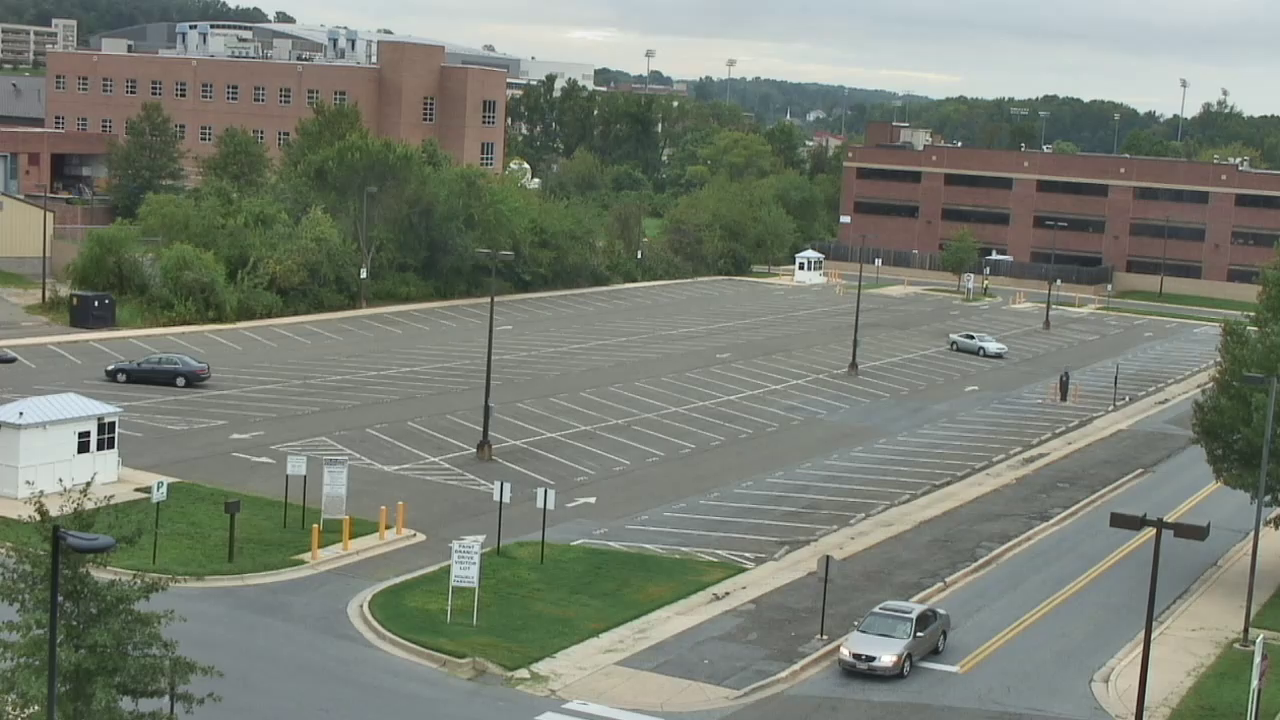
\includegraphics[width=.45\textwidth]{resources/methodology/original.png}\hfill
    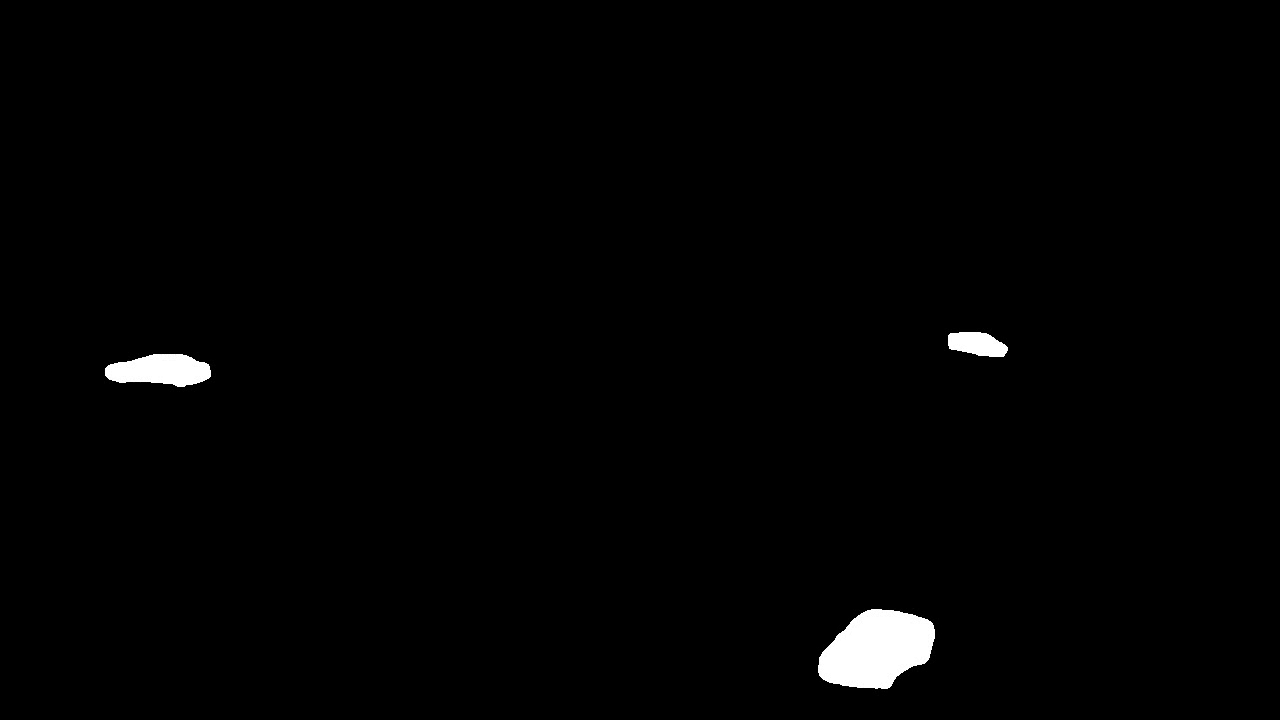
\includegraphics[width=.45\textwidth]{resources/methodology/car_segmentation.png}
    \caption{Segmentation result of cars}
    \label{fig:figure3}
\end{figure}
The idea is that the SP will learn to find an optimal general representation of cars. How general this representation is can be configured using the various parameters, but ideally they should be set so that different cars will be represented similarly while trucks and motorcycles will be represented differently. The task of the TM will then be to learn the common patterns that the cars exhibit, their speed, shape, and positioning will be taken into account. Finally, the learning will be set so that new patterns are learned quickly, but forgotten slowly. This will allow the system to quickly learn the norm, even if there is little activity, while still reacting to anomalies. \par
Ideally, the system will have a calibration period spanning several days or weeks, during which the system is not performing anomaly detection, but is just learning the patterns.\par
One issue that becomes evident is the lack of invariance. Because the TM is learning the global patterns, it learns that it is normal for cars to drive along the road but only in the context of there being cars parked in the parking lot. It is instead desired that the TM learns that it is normal for cars to drive along the road, regardless of whether there are cars in the parking lot. This thesis proposes a solution based on dividing the encoder output into a grid, and have a separate SP and TM for each cell in the grid. The anomaly scores of all the cells are then aggregated into a single anomaly score using an aggregation function e.g. the mean.
\begin{figure}[H]
    \centering
    \includegraphics[width=0.7\textwidth]{example-image-a}
    \caption{The encoder output divided into a grid.}
    \label{fig:grid}
\end{figure}
Another problem is that the previously mentioned rules for creating a good encoder may not be respected, and therefore should be reviewed:
\begin{itemize}
    \item \textbf{Semantically similar data should result in SDRs with overlapping active bits}. In this case, a car at the one position will produce an SDR with a high amount of overlapping bits as another car at a similar position in the input image.
    \item \textbf{The same input should always produce the same SDR}. The segmentation model produces a deterministic output given the same input.
    \item \textbf{The output must have the same dimensionality (total number of bits) for all inputs}. The segmentation model output has a fixed dimensionality.
    \item \textbf{The output should have similar sparsity (similar amount of one-bits) for all inputs and have enough one-bits to handle noise and subsampling}. The segmentation model does not respect this. An example is that there can be no cars (zero active bits), one car ($n$ active bits), or two cars ($2n$ active bits).
\end{itemize}
The solution for the last rule is two-fold, and  consists of imposing an upper bound and a lower bound for the number of active pixels within a cell with the purpose of lowering the variation of number of active pixels, while also containing enough semantic information for the HTM to work:
\begin{itemize}
    \item Pick a cell size so that the distribution of number of active pixels is as tight as possible, while containing enough semantic information and also being small enough so that the desired invariance is achieved. The cell size acts as an upper bound for the possible number of active pixels.
    \item Create a pattern representing emptiness, where the number of active bits is similar to what can be expected on average when there are cars inside a cell. This acts as a soft lower bound for the number of active pixels.
\end{itemize}
There could be situations where a few pixels are active within a cell, which could happen when a car has just entered a cell, but this is fine as long as it does not affect the distribution too much. In the following example, the number of active pixels within a cell centered in the video was used to build the following distributions:
\begin{figure}[H]
    \centering
    \begin{subfigure}[t]{0.5\textwidth}
        \centering
        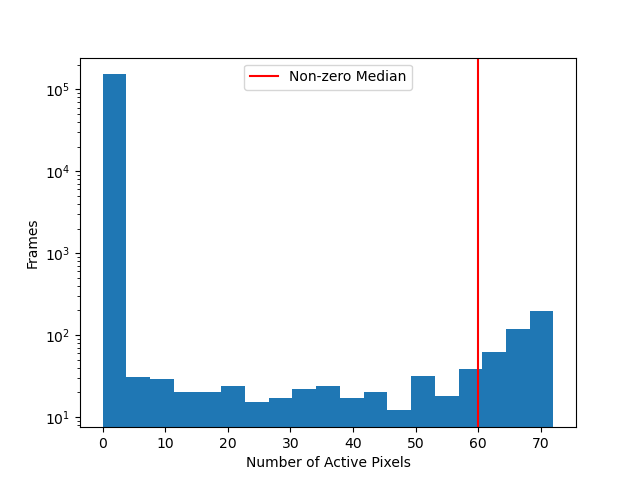
\includegraphics[width=\textwidth]{resources/methodology/active_pixels_dist.png}
        \caption{Without empty pattern.}
        \label{fig:num_active_pixels_cell}
    \end{subfigure}%
    \begin{subfigure}[t]{0.5\textwidth}
        \centering
        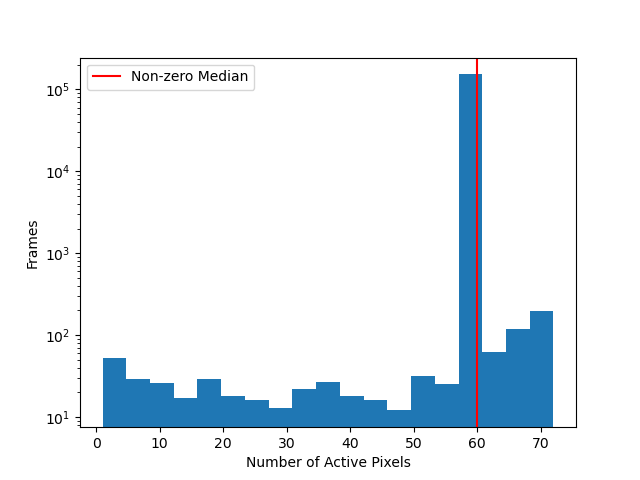
\includegraphics[width=\textwidth]{resources/methodology/active_pixels_dist2.png}
        \caption{With empty pattern.}
        \label{fig:num_active_pixels_cell2}
    \end{subfigure}
    \caption{Distribution of number of active pixels within a cell of size $12\times 12$}
    \label{fig:test}
\end{figure}


With a carefully selected empty pattern sparsity, \textbf{the standard deviation of active pixels was lowered from $\mathbf{3.78}$ to $\mathbf{1.88}$}. It is possible to automate this process by developing an algorithm which finds the optimal cell size and empty pattern sparsity which causes the least variation of number of active pixels per cell. This algorithm would be a part of the calibration process.
\begin{figure}[H]
    \centering
    \includegraphics[width=0.7\textwidth]{example-image-c}
    \caption{Encoder output.}
    \label{fig:encoder_output}
\end{figure}

